\documentclass[11pt]{article}

\usepackage{latexsym}
\usepackage{amsmath}
\usepackage{amssymb}
\usepackage{amsthm}
\usepackage{graphicx}
\usepackage{wrapfig}
\usepackage{pseudocode}
\usepackage{url}
\usepackage{listings}
\usepackage{xcolor}
\usepackage[backref, colorlinks=true, citecolor=red, urlcolor=blue, pdfauthor={Jyh-Ming Lien}]{hyperref}
\lstset {
    language=C,
                keywordstyle=\color{blue},
                stringstyle=\color{red},
                commentstyle=\color{green},
                morecomment=[l][\color{magenta}]{\#}
}


\newcommand{\handout}[5]{
  \noindent
  \begin{center}
  \framebox{
    \vbox{
      \hbox to 5.78in { {\bf Advanced Algorithms} \hfill #2 }
      \vspace{4mm}
      \hbox to 5.78in { {\Large \hfill #5  \hfill} }
      \vspace{2mm}
      \hbox to 5.78in { {\em #3 \hfill #4} }
    }
  }
  \end{center}
  \vspace*{4mm}
}

\newcommand{\lecture}[4]{\handout{#1}{#2}{#3}{}{#1}}

\newtheorem{theorem}{Theorem}
\newtheorem{corollary}[theorem]{Corollary}
\newtheorem{lemma}[theorem]{Lemma}
\newtheorem{observation}[theorem]{Observation}
\newtheorem{proposition}[theorem]{Proposition}
\newtheorem{definition}[theorem]{Definition}
\newtheorem{claim}[theorem]{Claim}
\newtheorem{fact}[theorem]{Fact}
\newtheorem{assumption}[theorem]{Assumption}

% 1-inch margins, from fullpage.sty by H.Partl, Version 2, Dec. 15, 1988.
\topmargin 0pt
\advance \topmargin by -\headheight
\advance \topmargin by -\headsep
\textheight 8.9in
\oddsidemargin 0pt
\evensidemargin \oddsidemargin
\marginparwidth 0.5in
\textwidth 6.5in

\parindent 0in
\parskip 1.5ex
%\renewcommand{\baselinestretch}{1.25}

\begin{document}

\lecture{Program Assignment 1 - 3D $\alpha$-shape}{Fall 2015}{Prof.\ Jyh-Ming Lien}{---}

152cpg04 \quad  Yunjoo Park

\href{mailto:yunjoopark12@gmail.com}{\it yunjoopark12@gmail.com}

git clone \href{https://github.com/yunjoopark/programmingAssignment1.git}{https://github.com/yunjoopark/programmingAssignment1.git}

\section{3D $\alpha$-shape}

\subsection{Problem definition and Analysis}
Let $P := \{p_1,p_2,...,p_n\}$ be a set of points in the plane. In that, an $\alpha$-shape of \textit{P} is the intersection of all closed circles with radius $\alpha$ that contain all the points. In other words, for a given value $\alpha$ and input as 3D, the $\alpha$-shape includes all the tetrahedra in the Delaunay Triangulation which have an empty circumsphere with \textit{squared radius} equal or smaller than $\alpha$. The value of $\alpha$ goes from $0 \rightarrow \infty$.
\begin{equation*}
\begin{cases} \alpha \rightarrow 0: \alpha$-shape is $P.\\
\alpha \rightarrow \infty: \alpha$-shape is$ \textit{CH(P)}.\\
\alpha \rightarrow 1: \alpha$-shape is a collection of triangles in$ \textit{DT(P)} $ whose circumcircles have diameters $ \leq \alpha.
\end{cases}
\end{equation*}
\subsection{Platforms}
Languages: C

Platform: Microsoft visual Studio 2013

\subsection{Examples of Inputs}
1. There are 11 test data.

2. Each data file has different values.

3. Each line has three value, $x, y, z$.

\clearpage

\subsection{Problem-solving methods and algorithms}
A tetrahedron is composed of four triangular faces. It has four faces, six edges, and four vertices. For all tetrahedron, there exists a sphere called 'circumsphere' which completely encloses the thetrahedron. All tetrahedron's vertices all lie on the surface of its circumsphere. The point at the centre of the circumsphere is the circumcentre. When the six edges of a tetrahedron are given, we can determine the radius of the circumsphere. Let the length of edges be $p, q, r, a, b, and c$. Let the $T$ be the volume of the tetrahedron and the radius of the sphere be $r$. Also, let the products of the opposite edge of the tetrahedron be $e = ap, f=bq, g = cr$ and the area of the triangle whose sides are products of these edges be $area$. Then, the radius $r$
\begin{equation*}
r = {area\over 6T}
\end{equation*}
We can calculate the area of the triangle whose sides have lengths a, b, and c by Heron's area formula.
\begin{equation*}
S = \sqrt{s(s-a)(s-b)(s-c)},
\end{equation*}
\begin{equation*}
s = {a + b + c \over 2}
\end{equation*}
Also, we can calcuate the volume of a tetrahedron with a function \textit{ Volumei(face, vertex)}.

\begin{lstlisting}
	volume = fabs(Volumei(&face, tetra->vertex[3]));
	
	if (facet->normal[3] < 0.0 && volume) {
		area = areaTriangle(tetra);
		radius = area / (6 * volume);
		
		if (radius < alpha) {
			tetra->face[0] = MakeFace(tetra->vertex[0], tetra->vertex[1], tetra->vertex[2], NULL);
			tetra->face[1] = MakeFace(tetra->vertex[3], tetra->vertex[1], tetra->vertex[0], NULL);
			tetra->face[2] = MakeFace(tetra->vertex[2], tetra->vertex[3], tetra->vertex[0], NULL);
			tetra->face[3] = MakeFace(tetra->vertex[1], tetra->vertex[2], tetra->vertex[3], NULL);
		}
	}

\end{lstlisting}
Since volume has sign, I made it into an absolute value. Then, calculate a radius and compare the radius with given value, alpha $\alpha$. Draw only tetrahedra with \textit{radius} equal or smaller than $\alpha$.

\subsection{Results Analysis and Discussion}
In this report, implement $\alpha$-shape algorithm by using \textit{qhull}. For determining the radius of a circumsphere, I have to calculate the area of the triangle which lengths of sides are the products of the opposite edge of the tetrahedron. I used Heron's area formula to compute the area. By reducing the value of $\alpha$, $\alpha$-shape exhibited the specific shape of the $P$. Finally,
\begin{equation*}
\lim_{\alpha \to 0}P_\alpha = P\\
\end{equation*}
\begin{equation*}
\lim_{\alpha \to \infty}p_\alpha = CH(P)
\end{equation*}

\subsection{Outputs}
\begin{figure}[ht]
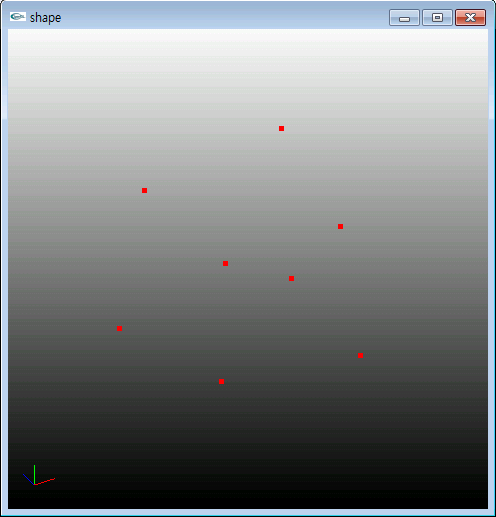
\includegraphics[width=.5\textwidth]{FIGS/alpha0-icube}
\hspace{1cm}
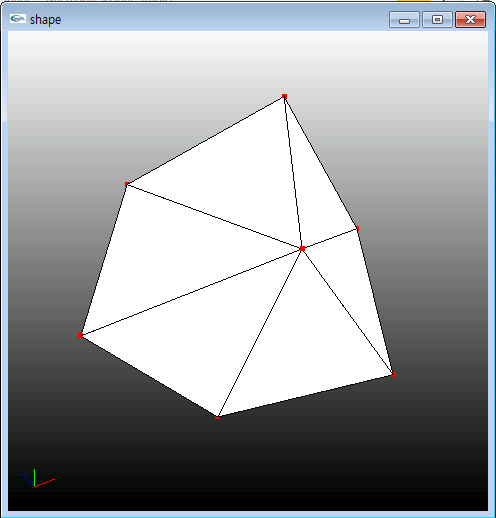
\includegraphics[width=.5\textwidth]{FIGS/alpha2-icube}
\vspace{1cm}
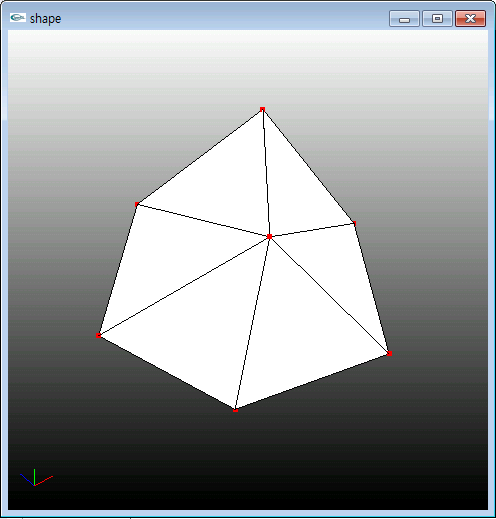
\includegraphics[width=.5\textwidth]{FIGS/alpha10-icube}
\caption{$\alpha$ = 0, $\alpha$ = 2, $\alpha$ = 10 \textit{i.cube}}
\end{figure}


\begin{figure}[ht]
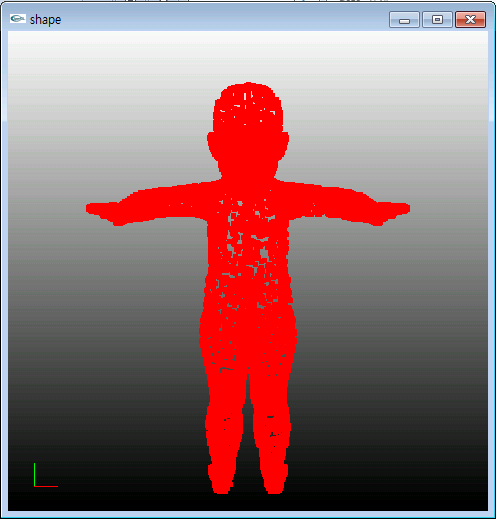
\includegraphics[width=.5\textwidth]{FIGS/alpha0-ibb}
\hspace{1cm}
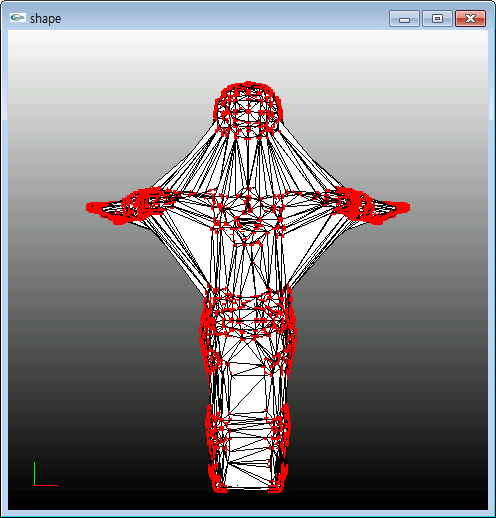
\includegraphics[width=.5\textwidth]{FIGS/alpha10-ibb}
\vspace{1cm}
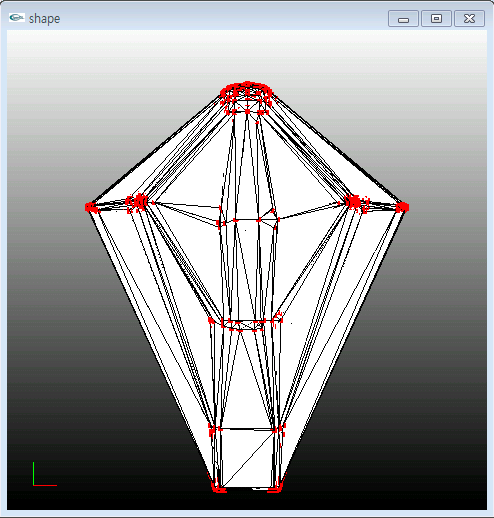
\includegraphics[width=.5\textwidth]{FIGS/alpha100-ibb}
\caption{$\alpha$ = 0, $\alpha$ = 10, $\alpha$ = 100 \textit{i.bb}}
\end{figure}


\begin{figure}[ht]
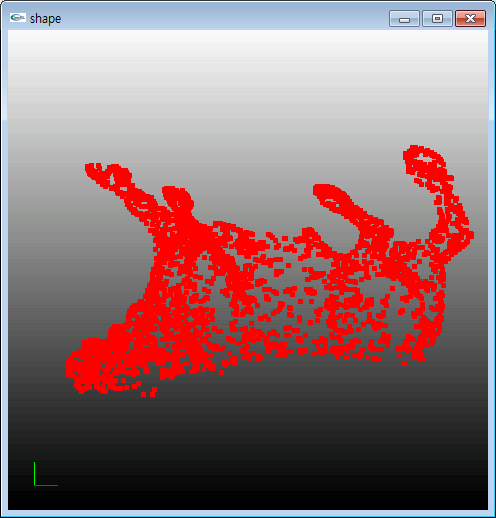
\includegraphics[width=.5\textwidth]{FIGS/alpha0-ibull}
\hspace{1cm}
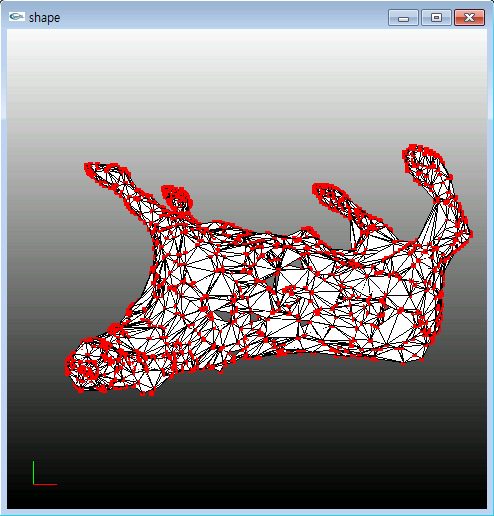
\includegraphics[width=.5\textwidth]{FIGS/alpha100-ibull}
\vspace{1cm}
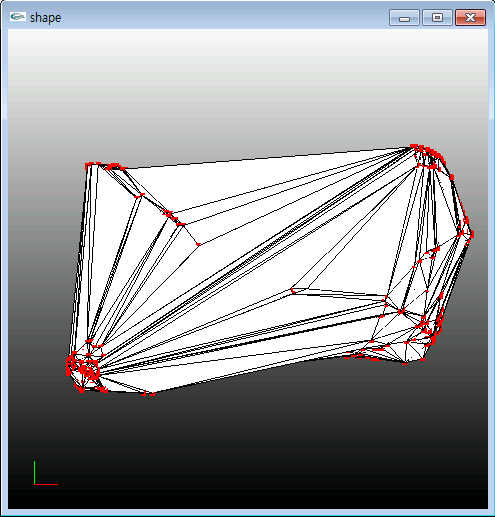
\includegraphics[width=.5\textwidth]{FIGS/alpha1000-ibull}
\caption{$\alpha$ = 0, $\alpha$ = 100, $\alpha$ = 1000 \textit{i.bull}}
\end{figure}


\end{document}


